\RequirePackage{mmap}
\documentclass[12pt]{article}
\usepackage[utf8]{inputenc}
\usepackage{geometry}
\geometry{
  margin=1in,
}
\usepackage{amsmath,amsthm,amssymb, listings, color}
\usepackage{mathtools}
\usepackage{changepage}% http://ctan.org/pkg/changepage
\usepackage{enumitem}
\usepackage{csquotes}
\usepackage{fancyhdr}
\usepackage[T1]{fontenc}
\usepackage{titlesec}
\usepackage[absolute]{textpos}
\usepackage[hidelinks]{hyperref}
\usepackage{fontspec}
\setmainfont{Latin Modern Roman}
%% \usepackage{setspace}
%% \doublespacing

\newcommand\defeq{\stackrel{\mathclap{\normalfont\mbox{\scriptsize def}}}{=}}
\newtheorem{theorem}{Theorem}[section]
\newtheorem{corollary}{Corollary}[theorem]
\newtheorem{lemma}[theorem]{Lemma}
\newtheorem{innercustomgeneric}{\customgenericname}
\providecommand{\customgenericname}{}
\newcommand{\newcustomtheorem}[2]{%
  \newenvironment{#1}[1]
  {%
   \renewcommand\customgenericname{#2}%
   \renewcommand\theinnercustomgeneric{##1}%
   \innercustomgeneric
  }
  {\endinnercustomgeneric}
}

\newcustomtheorem{customthm}{Theorem}
\newcustomtheorem{customlemma}{Lemma}
\newcustomtheorem{customdef}{Definition}

\newcommand{\istart}[1]{\underline{\textit{#1}}\\}
\newcommand{\idetail}[1]{\footnotesize\textbf{\emph{#1}}\normalsize}
\newcommand{\mapto}{\rightarrow}
\newcommand{\bR}{\mathbb{R}}

\setlength{\parindent}{0.25in}
\setlength{\parskip}{0.5em}

\newif\ifextra
\extrafalse

\title{}

\pagenumbering{arabic}

\begin{document}
\pagestyle{fancy}
\fancyhf{} % sets both header and footer to nothin
\cfoot{\thepage}
\renewcommand{\headrulewidth}{1pt}
\lhead{\fontsize{10}{12} \selectfont CSE 599: Convex Optimization and Geometry (Prof. Yin Tat Lee)\\\textbf{Summary of Lecture 2} }
\rhead{\fontsize{10}{12} \selectfont Kaiyu Zheng\\ \today}

This series of lecture summaries is to extract the key theorems and ideas from the lecture notes. I do not understand them all, but at least I condense the knowledge and do not need to read the lengthy lecture notes again.

\section{Cutting Plane Methods}
A set of lectures on the \emph{cutting plane method}, an iterative process, for solving convex optimization problems.
\begin{enumerate}
\item \istart{Intuition behind cutting plane methods} If $f$ is a continuously differentialble convex function, then:
  $$f(y)\geq f(x)+(\nabla f(x))^T(y-x)$$
  Suppose $x^*$ is the minimizer of $f$ (i.e. $f(x)\geq f(x^*)$ for all $x$). Then,
  $$f(x)\geq f(x^*)\geq f(x) + (\nabla f(x))^T(x^*-x)$$
  Therefore, $(\nabla f(x))^T(x^*-x)\leq 0$. Thus, $x^*$ lies on the half space with normal $-\nabla f(x)$.
  \begin{figure}[h]
    \centering
    \includegraphics[scale=0.5]{figs/cutting}
    \caption{Half space containing the minimizer after one iteration of the cutting plane method.}
    \label{fig:cutting}
  \end{figure}
  
  \idetail{Note} You should not interpret $(\nabla f(x))^T(x^*-x)$ as a hyperplane and $\nabla f(x)$ as the normal vector, because both $f(x)$ and $(x^*-x)$ are fixed vectors (instead of vector dot product with a point). But $\nabla f(x))$ definitely defines a hyperplane, as indicated by the purple line in the diagram.

\item \istart{Minimizer is in a half space}
  Any minimizer $x^*$ lies in the half space
  $$H^{(k)}\defeq\{x\in\bR^n: (\nabla f(x))^T(x^*-x)\leq 0\}$$
  This half space is the entire region above the purple line in the diagram. And let $E^{(k)}$ be a convex set that definitely contains $x^*$. Then, $x^*\in H^{(k)}\cap E^{(k)}$.
\end{enumerate}

\item \istart{Ellipsoid Method}
%% \bibliography{references}
%% \bibliographystyle{plain}

\end{document}


